% =============================================================================
% dev_tool.tex — The Solanus Casey archival DEV TOOL, explained from first
% principles. Wording follows the comments in app/server.py, app/static/*,
% app/tools/*, and eval/eval.py so this reads as a clean, polished version of
% the same explanation.
%
% Build (keeps ALL aux files in build/):
%     latexmk -pdf -outdir=build dev_tool.tex
% so only dev_tool.tex and build/dev_tool.pdf exist (copy the pdf up if you
% want it beside the source). Nothing exotic is required beyond a TeX Live
% with tikz + tcolorbox.
% =============================================================================
\documentclass[11pt]{article}
\usepackage{lmodern}
\usepackage[T1]{fontenc}

% --- Packages ---------------------------------------------------------------
\usepackage[margin=1in]{geometry}
\usepackage{amsmath, amssymb}
\usepackage{graphicx}
\usepackage{booktabs}
\usepackage{microtype}
\microtypesetup{expansion=false}
\usepackage{enumitem}
\usepackage{xcolor}
\usepackage{hyperref}
\usepackage{listings}
\usepackage{tikz}
\usepackage[most]{tcolorbox}
\usetikzlibrary{arrows.meta, positioning, decorations.pathreplacing,
                calc, shapes.geometric, patterns, fit, backgrounds}
\usepackage{placeins}   % \FloatBarrier to keep figures inside their section
\usepackage{caption}
\captionsetup{font=small, skip=8pt}

\hypersetup{colorlinks=true, linkcolor=blue!50!black,
            urlcolor=blue!50!black, citecolor=blue!50!black}

% --- The two example boxes (numbers / primer), kept identical in spirit -----
\newtcolorbox{numbersbox}[1][]{
  colback=blue!5, colframe=blue!50!black, fonttitle=\bfseries,
  title={#1}, sharp corners, boxrule=0.6pt}

\newtcolorbox{primerbox}[1][]{
  colback=yellow!10, colframe=orange!70!black, fonttitle=\bfseries,
  title={#1}, sharp corners, boxrule=0.6pt}

% A warm "key idea" callout in the Capuchin brown of the app's own theme.css.
\definecolor{provincial}{RGB}{60,22,5}
\newtcolorbox{ideabox}[1][]{
  colback=provincial!5, colframe=provincial!70!black, fonttitle=\bfseries,
  title={#1}, sharp corners, boxrule=0.6pt}

% --- Listings (JSON / Python), muted like the diffusion explainer -----------
\definecolor{codebg}{RGB}{248,248,248}
\definecolor{codekw}{RGB}{0,0,180}
\definecolor{codecmt}{RGB}{0,128,0}
\definecolor{codestr}{RGB}{170,55,0}
\lstset{
  basicstyle=\ttfamily\small,
  backgroundcolor=\color{codebg},
  keywordstyle=\color{codekw}\bfseries,
  commentstyle=\color{codecmt}\itshape,
  stringstyle=\color{codestr},
  showstringspaces=false,
  breaklines=true,
  columns=fullflexible,
  frame=single,
  framesep=4pt,
  rulecolor=\color{black!20},
}

\newcommand{\code}[1]{\texttt{#1}}

\title{The Dev Tool: a glass-box agent over Father Solanus Casey's archive}
\author{Solanus Project Pipeline --- step\_7}
\date{}

\begin{document}
\maketitle
\tableofcontents
\bigskip

%==============================================================================
\section{TL;DR}
%==============================================================================

\begin{ideabox}[The one-sentence version]
The dev tool is a web app that answers questions about Father Solanus Casey's
$\sim$570 letters and $\sim$716 notebook pages with \textbf{grounded, cited}
prose --- and lets you \textbf{watch every step the machine took}, while
swapping the model that did it. It is a glass box, not a black box.
\end{ideabox}

\begin{itemize}[leftmargin=1.4em]
  \item \textbf{Three model choices are \emph{variables}}, picked from dropdowns:
        the \textbf{LLM} (generation), the \textbf{embedding space} (retrieval),
        and the \textbf{reranker}. Swap one, re-ask, compare. That loop is the
        whole instrument.
  \item \textbf{Retrieval is a row of toggles} --- BM25, dense, rerank, HyDE,
        multi-query, the LLM router. In the agent path the same idea becomes
        \textbf{toggleable tools}: \code{vector\_search}, \code{pdf\_fulltext\_search},
        \code{entity\_lookup}, \code{graph\_query}, \code{temporal\_query},
        \code{community\_summary}.
  \item \textbf{Every claim cites the exact handwritten region.} Click a
        \texttt{[1]} and a deep-zoom IIIF viewer opens the scan, boxes the cited
        region, and offers a \emph{Download source PDF} button.
  \item \textbf{A knowledge-graph view} renders people, places, records and their
        relations; clicking a record opens its scan.
  \item \textbf{Observability + evaluation are first-class}: every request
        returns a trace and a running cost ledger; an offline harness scores
        whole \emph{configurations} on RAGAS-style metrics so you pick a winner
        empirically.
  \item \textbf{Nothing bills you by accident.} The local path costs \$0; every
        paid touchpoint routes through \code{lib/costlog.py} and is gated.
\end{itemize}

%==============================================================================
\section{The mental model: one settings object, made visible}
%==============================================================================

The cleanest way to hold the whole tool in your head is this: \textbf{the left
rail of the UI is a live picture of one \code{RetrievalConfig}} (the same
dataclass \code{lib/retrieval.py} uses). Every dropdown and every toggle does
exactly one thing --- it sets a field on that object. When you press
\textbf{Ask}, the object is serialized and POSTed to the backend; the configured
retrieval runs \emph{once}; an LLM writes a cited answer; and the page renders
four things at once: the answer, its citations, the trace, and the cost.

\begin{ideabox}[Why this design earns its keep]
Because the only thing that changes between two questions is the \emph{settings
object}, you can do real science: hold the question fixed, flip one toggle or
swap one model, ask again, and read the difference straight off the trace and
the eval. The tool is built so that ``change one variable, observe'' is the
\emph{easiest} thing to do.
\end{ideabox}

There are two answer paths, and the server (\code{app/server.py}) speaks both,
because they answer two different research questions.

\begin{figure}[h]
\centering
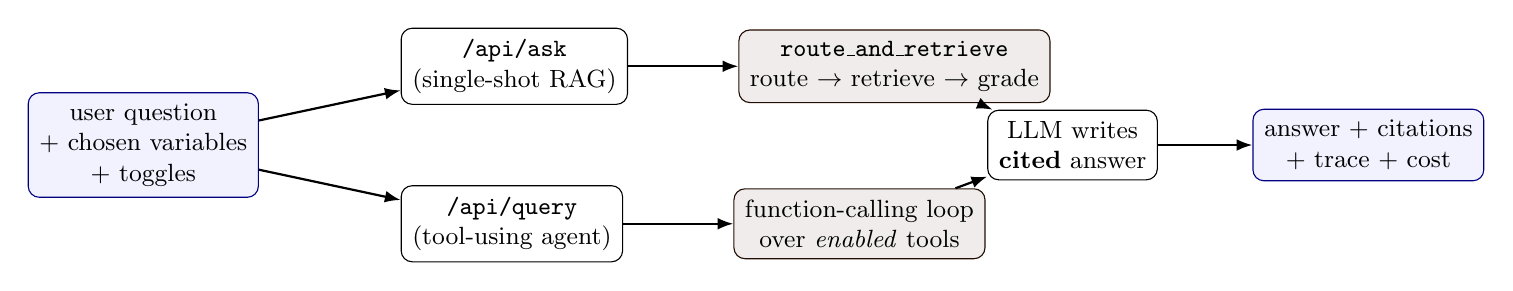
\begin{tikzpicture}[
   node distance=6mm and 12mm,
   box/.style={draw, rounded corners, align=center, minimum height=8mm,
               inner sep=4pt, font=\small},
   lib/.style={box, fill=provincial!8, draw=provincial!60!black},
   io/.style={box, fill=blue!5, draw=blue!50!black},
   arr/.style={-{Latex[length=2mm]}, thick}]

  \node[io] (q) {user question \\ + chosen variables \\ + toggles};

  \node[box, right=18mm of q, yshift=10mm] (ask) {\code{/api/ask}\\(single-shot RAG)};
  \node[box, right=18mm of q, yshift=-10mm] (query) {\code{/api/query}\\(tool-using agent)};

  \node[lib, right=14mm of ask] (route) {\code{route\_and\_retrieve}\\route $\to$ retrieve $\to$ grade};
  \node[lib, right=14mm of query] (loop) {function-calling loop\\over \emph{enabled} tools};

  \node[box, right=14mm of $(route)!0.5!(loop)$] (gen) {LLM writes\\\textbf{cited} answer};

  \node[io, right=12mm of gen] (out) {answer + citations\\+ trace + cost};

  \draw[arr] (q) -- (ask);
  \draw[arr] (q) -- (query);
  \draw[arr] (ask) -- (route);
  \draw[arr] (query) -- (loop);
  \draw[arr] (route) -- (gen);
  \draw[arr] (loop) -- (gen);
  \draw[arr] (gen) -- (out);
\end{tikzpicture}
\caption{Two paths, one discipline. \code{/api/ask} runs a single toggle-driven
retrieval then synthesizes; \code{/api/query} lets the model loop over toggleable
tools. Both ground every claim, abstain when evidence is thin, cite
\code{doc\_id+rid+page+vertices}, and cost-log every model touch.}
\end{figure}

\FloatBarrier

%==============================================================================
\section{A brief jargon primer}
%==============================================================================
Skip if RAG, an embedding space, a reranker, and function-calling are already
old friends.

\begin{primerbox}[Retrieval-Augmented Generation (RAG), in one breath]
A language model is fluent but forgetful and prone to confident invention. RAG
fixes that by \emph{retrieving} the relevant passages from a trusted corpus
first, then asking the model to answer \emph{only from those passages}. For an
archive this is non-negotiable: we want the friar's own words, not the model's
paraphrase of the internet.
\end{primerbox}

\paragraph{Embedding space.} An \emph{embedding} turns a passage into a vector
(a point in high-dimensional space) so that similar meanings sit near each
other. A \emph{space} is a particular (model, dimension) pair, e.g.
\code{gemini-embedding-001@1536}. Dense retrieval = ``find the passages whose
vectors point in nearly the same direction as the question's vector'' (cosine
similarity). Different spaces draw the map differently, which is exactly why we
make the space a swappable variable and \emph{measure} which one is best for
\emph{this} corpus.

\paragraph{BM25 (lexical).} The classic keyword score: a passage ranks high if
it literally contains the query's rare words. It is unbeatable for exact strings
--- a name like \emph{O'Donnell}, a year like \emph{1933} --- and it is free and
local. We fuse it with dense retrieval (via reciprocal-rank fusion) so we get
both ``means the same thing'' and ``says the same word''.

\paragraph{Reranker.} A fusion list is good but coarse. A \emph{cross-encoder}
reranker reads the question and each candidate \emph{together} and re-orders the
top handful for a sharper final ranking. It is the most accurate and the most
expensive step per item, so it is off by default and a toggle.

\paragraph{HyDE / multi-query.} Two cheap recall boosters. \textbf{HyDE} embeds a
\emph{hypothetical answer} (the model imagines what a good answer looks like, and
we search with \emph{that}), which often lands closer to the real passage than
the terse question does. \textbf{Multi-query} (RAG-Fusion) asks the same thing a
few different ways and fuses the results --- handy when notebook entries are
written in one register and your question in another.

\paragraph{Function-calling (tool use).} Modern LLMs can be handed a menu of
``tools'' (each a name + description + JSON parameter schema). Instead of
answering immediately, the model can \emph{call} a tool; we run it, hand back the
result, and let the model continue. The agent path is just this menu plus a loop.

\paragraph{Self-RAG / CRAG grade, and abstention.} Before trusting retrieved
context, we \emph{grade} it: does it actually support an answer? The verdict is
\textbf{answer}, \textbf{caveat}, or \textbf{abstain}. In an archive,
\emph{``I could not find this''} is a correct and valuable answer, so abstaining
on weak evidence is a feature, not a failure.

%==============================================================================
\section{The swappable axes (the variables)}
%==============================================================================

The UI does not hard-code its options; it builds itself from
\code{GET /api/config}, which reports the available LLMs (\code{config.LLMS}),
\textbf{only the embedding spaces that have a built partition}
(\code{vectorstore.spaces()}), and the rerankers (\code{config.RERANKERS}). That
last point is a small honesty win: the embedding dropdown can never offer a
partition you cannot actually search.

\begin{ideabox}[The human picks the variables; the model never does]
In the agent loop, \code{\_inject\_request\_variables} threads the chosen
embedding space / reranker into \code{vector\_search}'s arguments and the chosen
LLM into \code{community\_summary} --- \emph{behind} the model's back. So the
model's entire decision surface is ``what should I search for?'', never ``which
embedding model should I use?''. Shrinking the model's choices is what makes its
tool-use reliable.
\end{ideabox}

%==============================================================================
\section{The toggleable tools (the agent's powers)}
%==============================================================================

Each capability lives in its own file under \code{app/tools/} and registers a
single \code{Tool} --- a name, the description \emph{the model reads to decide
when to call it}, a JSON-Schema for its arguments, and the Python callable. The
payoff of one-file-per-tool: \textbf{adding a power is dropping a file that calls
\code{register(...)}}, and it shows up everywhere (UI switch, function-calling
schema, trace) with zero edits to the server.

\begin{numbersbox}[The registered tools (app/tools/)]
\centering\small
\begin{tabular}{lllc}
\toprule
tool & answers & default & cost \\
\midrule
\code{vector\_search}        & ``which passages match?''        & on  & free local; hosted = paid \\
\code{pdf\_fulltext\_search} & exact-string page search (FTS5)  & on  & free, local \\
\code{entity\_lookup}        & name $\to$ canonical entity      & on  & free, local \\
\code{temporal\_query}       & dates / timelines (EDTF)         & on  & free, local \\
\code{graph\_query}          & relational hops on the KG        & off & free local (needs graph) \\
\code{community\_summary}    & whole-corpus themes              & off & free digests; summary = paid \\
\bottomrule
\end{tabular}
\end{numbersbox}

\noindent The two \code{default\_on=False} tools are off \emph{honestly}: their
artifacts (\code{data/graph.json}; the community index) must be built first, and
``an honest UI never offers a switch that can't fire.'' A tool that raises never
kills the turn --- \code{tools.call(...)} wraps every invocation and returns a
structured \code{\{ok:false, error:\dots\}} the agent and the trace panel can read
and recover from.

\begin{primerbox}[A concrete Solanus example]
Ask \emph{``Which favors were reported for cancer?''} with \code{vector\_search}
on. The agent searches \emph{cancer cure reported}, and gets back notebook
entries each carrying provenance --- e.g.\ \code{doc\_id=Volume\_6\_\_p178},
\code{rid=doc\_1.src\_content.0}, \code{pdf\_page=183}, and the gold polygon
\code{vertices} --- then answers with \texttt{[1]\dots[n]} markers. Now toggle on
\code{graph\_query} and ask \emph{``What continues onto page 178?''}: the agent
walks a \code{CONTINUES\_ON} edge and cites \emph{both} fragments. Same archive,
a different power switched on.
\end{primerbox}

%==============================================================================
\section{The agent loop and the router}
%==============================================================================

The function-calling loop in \code{agent\_query} is small on purpose:

\begin{enumerate}[leftmargin=1.6em]
  \item Seed the conversation with the question; the \textbf{system prompt}
        carries the grounding + citation + abstain policy.
  \item Ask the model, offering \textbf{only the enabled tools'} declarations.
        It either \emph{calls} tools or \emph{answers}.
  \item For each call: run the tool (error-wrapped), \textbf{record a trace
        span}, \textbf{harvest provenance into citations}, remember the best
        retrieval \textbf{grade}, append the result to history.
  \item Repeat until it answers or hits \code{max\_steps} --- a safety cap so a
        confused model cannot loop forever and run up cost.
\end{enumerate}

\begin{figure}[h]
\centering
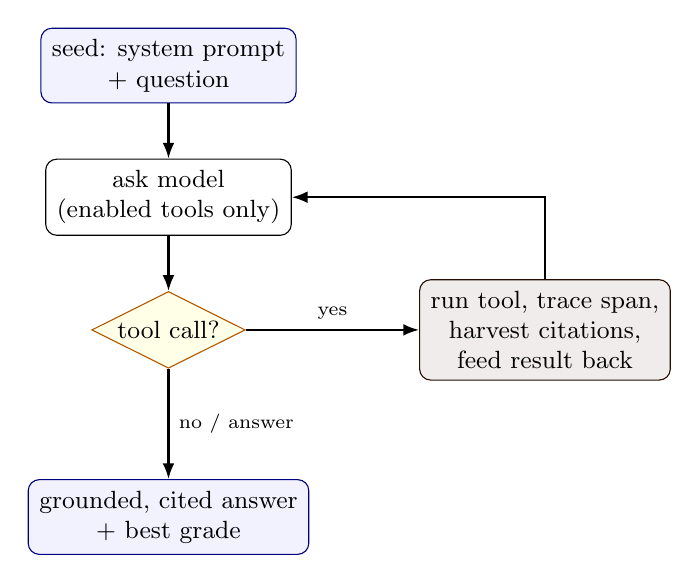
\begin{tikzpicture}[
   node distance=7mm,
   box/.style={draw, rounded corners, align=center, font=\small, inner sep=4pt,
               minimum height=8mm},
   dec/.style={draw, diamond, aspect=2, align=center, font=\small,
               inner sep=1pt, fill=yellow!10, draw=orange!70!black},
   arr/.style={-{Latex[length=2mm]}, thick}]

  \node[box, fill=blue!5, draw=blue!50!black] (seed) {seed: system prompt\\+ question};
  \node[box, below=of seed] (ask) {ask model\\(enabled tools only)};
  \node[dec, below=of ask] (d) {tool call?};
  \node[box, right=22mm of d, fill=provincial!8, draw=provincial!60!black]
       (tool) {run tool, trace span,\\harvest citations,\\feed result back};
  \node[box, below=14mm of d, fill=blue!5, draw=blue!50!black]
       (answer) {grounded, cited answer\\+ best grade};

  \draw[arr] (seed) -- (ask);
  \draw[arr] (ask) -- (d);
  \draw[arr] (d) -- node[above, font=\scriptsize]{yes} (tool);
  \draw[arr] (tool) |- (ask);
  \draw[arr] (d) -- node[right, font=\scriptsize]{no / answer} (answer);
\end{tikzpicture}
\caption{The agent loop. The cycle back to ``ask model'' is capped by
\code{max\_steps} so cost is always bounded.}
\end{figure}

\FloatBarrier

In the single-shot path the equivalent ``thinking'' is the \textbf{adaptive
router}: \code{route\_and\_retrieve} classifies the query's complexity and picks
a strategy (simple $\to$ direct lexical; complex $\to$ fan-out + fuse), then the
CRAG-style grade decides \emph{answer / caveat / abstain}. The trace shows the
route decision on its own line, so you can see \emph{why} the system spent (or
chose not to).

%==============================================================================
\section{Citations: the IIIF modal + PDF download}
%==============================================================================

This is the heart of ``provenance-first.'' A citation here is not a footnote
string; it is a \textbf{clickable pointer to pixels}. Clicking \texttt{[1]} (or a
source row, or a record node in the graph) calls
\code{GET /api/region?doc\_id=\dots\&rid=\dots}, which the server resolves from
the step\_6 source records: the region's \textbf{text}, its gold polygon
\textbf{\code{vertices}}, the OCR \textbf{\code{min\_conf}}, the page \textbf{PNG}
(\code{/api/image/...}), the \textbf{searchable PDF} (\code{/api/pdf/...},
preferring the text-layer copy), and the \textbf{IIIF manifest}
(\code{/api/manifest/...}). The front-end then deep-zooms the scan with
OpenSeadragon, converts the pixel \code{vertices} into viewport coordinates,
\emph{draws a highlight box} (dimming the rest of the page), frames the region,
and wires the \emph{Download source PDF} button.

\begin{figure}[h]
\centering
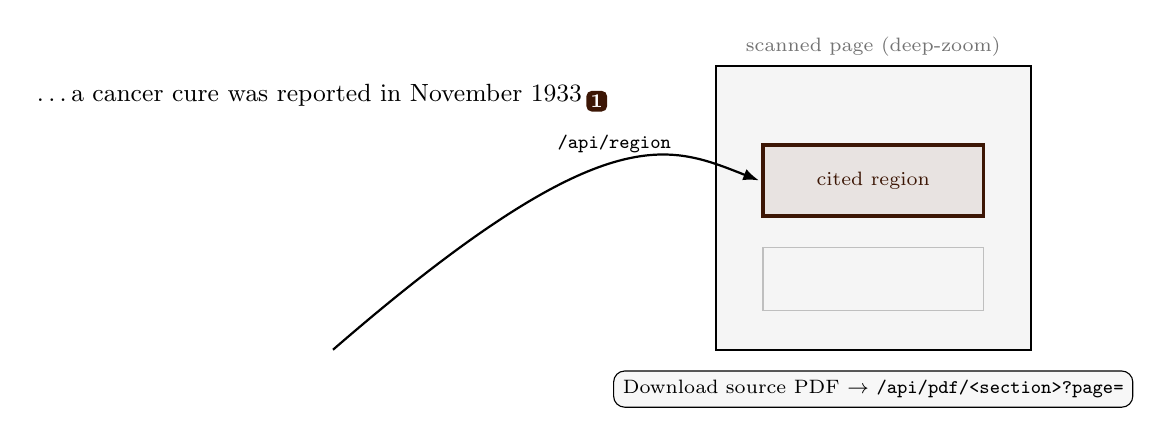
\begin{tikzpicture}[scale=1.0]
  % "the answer" with a clickable [1]
  \node[align=left, font=\small] (ans) at (0,3.2)
    {\dots a cancer cure was reported in November 1933\,%
     \tikz[baseline]{\node[fill=provincial, text=white, font=\scriptsize\bfseries,
        rounded corners=2pt, inner sep=1.5pt] (cite) {1};}};

  % the scanned page
  \draw[thick, fill=black!4] (5,0) rectangle (9,3.6);
  \node[font=\scriptsize, text=black!55] at (7,3.85) {scanned page (deep-zoom)};
  % the highlighted region (the "vertices" box)
  \draw[provincial, very thick, fill=provincial!12]
        (5.6,1.7) rectangle (8.4,2.6);
  \node[font=\scriptsize, provincial] at (7,2.15) {cited region};
  % faint "other regions"
  \draw[black!25] (5.6,0.5) rectangle (8.4,1.3);

  % arrow: click [1] -> /api/region -> box on page
  \draw[-{Latex[length=2mm]}, thick]
        (cite.east) .. controls (3.6,3.0) and (4.4,2.6) ..
        node[above, font=\scriptsize]{\code{/api/region}} (5.55,2.15);

  % the PDF button
  \node[draw, rounded corners, font=\scriptsize, fill=black!3] at (7,-0.5)
       {Download source PDF $\to$ \code{/api/pdf/<section>?page=}};
\end{tikzpicture}
\caption{Click \texttt{[1]} $\to$ \code{/api/region} returns text + polygon +
image/PDF/manifest URLs $\to$ OpenSeadragon boxes the exact handwritten region
and the footer links the page's searchable PDF.}
\end{figure}

\FloatBarrier

\begin{ideabox}[Two safety habits worth copying]
The modal \textbf{degrades gracefully}: if the backend is offline or a PDF was
never generated, it shows what the citation already carries plus a friendly note,
instead of breaking. And it \textbf{never \code{innerHTML}s model output} --- the
LLM's text is untrusted, so \texttt{[n]} markers are parsed into DOM chips to
avoid an XSS hole. An archive tool that mishandles untrusted text is a liability,
not a convenience.
\end{ideabox}

%==============================================================================
\section{The knowledge-graph view}
%==============================================================================

\code{GET /api/graph} serves \code{data/graph.json} (built on demand if networkx
is present). The UI renders it with Cytoscape.js: nodes are letters, notebook
pages/entries, and resolved entities (person / place / org / condition / outcome
/ event), each brand-tinted by kind; edges are asserted relations
(\code{WROTE\_TO}, \code{LOCATED\_AT}, \code{CONTINUES\_ON}, \dots). There is an
\emph{entities-only} filter, \emph{fit} / \emph{reload} controls, and a legend.
Clicking an \textbf{entity} prints an inspect line (label, aliases, mention
count); clicking a \textbf{record} node opens its scan in the \emph{same}
citation modal. The graph is therefore a navigable index back into the page
images --- not a decorative blob.

\begin{figure}[h]
\centering
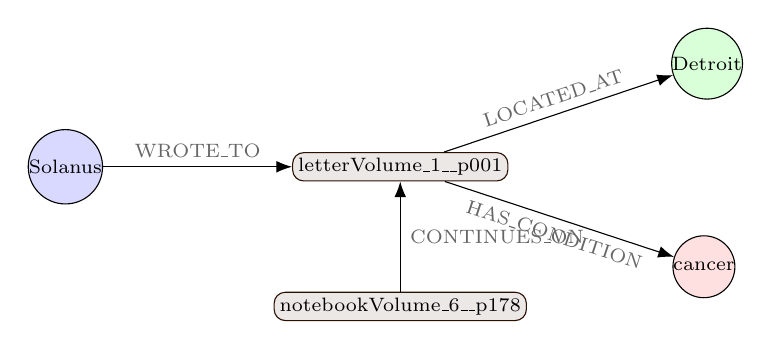
\begin{tikzpicture}[
   ent/.style={circle, draw, minimum size=7mm, font=\scriptsize, inner sep=0pt},
   rec/.style={rectangle, rounded corners, draw, font=\scriptsize, inner sep=2pt,
               fill=provincial!10, draw=provincial!70!black},
   rel/.style={font=\scriptsize, text=black!60}]
  \node[ent, fill=blue!15] (sol) {Solanus};
  \node[rec, right=24mm of sol] (let) {letter\\Volume\_1\_\_p001};
  \node[ent, fill=green!15, above right=8mm and 22mm of let] (det) {Detroit};
  \node[ent, fill=red!12, below right=8mm and 22mm of let] (cond) {cancer};
  \node[rec, below=14mm of let] (nb) {notebook\\Volume\_6\_\_p178};

  \draw[-{Latex[length=2mm]}] (sol) -- node[rel, above]{WROTE\_TO} (let);
  \draw[-{Latex[length=2mm]}] (let) -- node[rel, above, sloped]{LOCATED\_AT} (det);
  \draw[-{Latex[length=2mm]}] (let) -- node[rel, below, sloped]{HAS\_CONDITION} (cond);
  \draw[-{Latex[length=2mm]}] (nb) -- node[rel, right]{CONTINUES\_ON} (let);
\end{tikzpicture}
\caption{A few hops of the archival graph. Click ``cancer'' to inspect the
entity; click ``notebook Volume\_6\_\_p178'' to open its scan --- the same modal
the citations use.}
\end{figure}

\FloatBarrier

%==============================================================================
\section{Observability and evaluation}
%==============================================================================

\subsection{Per-request observability (the ``under the hood'' panel)}

The tool's whole pitch is ``see under the hood,'' so every request returns a
\textbf{trace}. Ideally those are OpenTelemetry spans flowing to \textbf{Arize
Phoenix} (OpenInference is the LLM-semantics layer Phoenix reads); if that stack
imports, the server registers a tracer provider and an exporter configured via
the standard \code{OTEL\_*} env vars picks the spans up. But we refuse to
\emph{depend} on a heavy optional stack --- so if it is absent, a dependency-free
\code{\_JsonTracer} records every step (\code{agent\_start}, each
\code{llm\_turn}, each \code{tool\_call} with latency, \code{agent\_end}),
returns it \emph{inline} as the response \code{trace}, and appends one JSONL line
to \code{app/traces/agent\_traces.jsonl}. Either way the panel works with zero
extra deps, and tracing is best-effort so it can never break a request.

\subsection{Offline evaluation: which knobs actually win?}

Once you can retrieve and answer, the hard question is \emph{which configuration
to ship}. \code{eval/eval.py} is the scoreboard. It runs a set of \textbf{golden
questions} through the real stack and scores the four metrics the RAG-eval
literature has settled on.

\begin{primerbox}[The four metrics, intuition first (the RAGAS/ARES playbook)]
\begin{itemize}[leftmargin=1.2em]
  \item \textbf{Faithfulness} --- ``does the answer actually follow from the
        retrieved context, or did the model invent it?'' Decompose the answer
        into atomic claims; score = supported claims / all claims. In an archive
        an unsupported claim is the cardinal sin, so this is the headline number.
  \item \textbf{Context precision} --- of the passages we retrieved, what
        fraction are relevant? (Don't drown the generator in noise.)
  \item \textbf{Context recall} --- of the passages we \emph{should} have
        retrieved, what fraction did we get? (Don't miss the evidence.)
  \item \textbf{Answer relevancy} --- does the answer address the question that
        was \emph{asked} (vs.\ true-but-off-topic)?
\end{itemize}
\end{primerbox}

\noindent A configuration \emph{passes} only if its mean clears \emph{every}
threshold --- intentionally strict, because we would rather flag a borderline
config than ship a confabulating one.

\begin{numbersbox}[Thresholds (RESEARCH\_PLAN Part E)]
\centering\small
\begin{tabular}{lc}
\toprule
metric & pass bar \\
\midrule
faithfulness       & $\ge 0.75$ \quad(headline) \\
context precision  & $\ge 0.70$ \\
context recall     & $\ge 0.80$ \\
answer relevancy   & $\ge 0.70$ \\
\bottomrule
\end{tabular}
\end{numbersbox}

The harness scores these for \textbf{every} $\{\text{LLM} \times
\text{embedding} \times \text{reranker}\}$ combination (\code{--sweep}) and
writes a ranked leaderboard to \code{data/eval\_results.json} with a per-config
verdict. There are \textbf{two grading backends}: a deterministic \emph{free
heuristic} (the default --- claim-splitting + lexical-overlap support, \$0) and a
\emph{RAGAS-faithful LLM judge} (paid, double-gated behind
\code{--use-llm-judge --i-accept-cost}). An ARES-style \emph{synthetic} question
generator exists too, but --- per project rule that gold is David's authority ---
it writes to a separate review file and is \emph{never} auto-merged into the gold
set.

%==============================================================================
\section{How to run it}
%==============================================================================

\begin{lstlisting}[language=bash]
# from the repo root -- add the two web deps to the step_7 venv (one-time)
pipeline_v3/step_7/venv/bin/pip install "fastapi>=0.110" "uvicorn[standard]>=0.29"

# (optional) observability -- else the JSON-tracer fallback is used automatically
# pip install opentelemetry-sdk opentelemetry-api openinference-instrumentation arize-phoenix

# launch the API + UI (this SERVES the app; do not run it as part of a build)
pipeline_v3/step_7/venv/bin/uvicorn app.server:app --reload --port 8000
#   -> open http://localhost:8000

# FREE offline self-check (no server, no paid call) -- confirms what is wired:
pipeline_v3/step_7/venv/bin/python app/server.py

# FREE eval (heuristic metrics, default config); --sweep compares all combos:
pipeline_v3/step_7/venv/bin/python eval/eval.py --sweep
\end{lstlisting}

%==============================================================================
\section{Caveats}
%==============================================================================

\begin{itemize}[leftmargin=1.4em]
  \item \code{fastapi} + \code{uvicorn} are \textbf{required and not yet
        installed}. The server imports them lazily; if missing,
        \code{app.server:app} becomes a stub that returns an actionable 500
        telling you what to install --- so \code{import app.server} still works
        for tests/inspection.
  \item \code{/api/query} and \code{/api/ask} \textbf{make paid LLM calls} (the
        agent reasons; the synthesizer writes). Retrieval is free with the local
        embedding + reranker variables; a hosted embedding space, a paid
        reranker, or any paid toggle (rerank / HyDE / multi-query / LLM-router)
        spends --- and is cost-logged. Nothing bills until you ask.
  \item Some tools \textbf{depend on upstream artifacts}: \code{graph\_query}
        needs \code{data/graph.json} (run \code{stages/build\_graph.py}, install
        networkx); \code{temporal\_query} needs \code{data/dates.json};
        \code{community\_summary}'s paid path needs the community index. These
        default OFF or degrade to a well-formed empty result.
  \item OpenTelemetry/Phoenix is \textbf{optional}; without it you still get the
        full inline JSON trace, just not the exportable Phoenix timeline.
  \item The eval metrics are \textbf{proxies on the free path} (lexical overlap,
        \code{expected\_where} slices); treat the free leaderboard as a relative
        A/B and enable the gated LLM judge for sharper absolute numbers.
\end{itemize}

%==============================================================================
\section{Sources / where to read next}
%==============================================================================

\begin{itemize}[leftmargin=1.4em]
  \item \textbf{Backend:} \code{app/server.py} (agent loop, \code{/api/*}, region
        resolution, observability fallback); \code{app/tools/base.py} (the
        \code{Tool} contract + registry); the six tool modules in
        \code{app/tools/}.
  \item \textbf{Front-end:} \code{app/static/index.html} (the five panes);
        \code{app/static/app.js} (rail $\to$ request, citation modal, graph);
        \code{app/static/theme.css}.
  \item \textbf{Retrieval brain + eval:} \code{lib/retrieval.py}
        (\code{RetrievalConfig}, \code{route\_and\_retrieve}, the grade);
        \code{eval/eval.py} (RAGAS/ARES metrics + the sweep);
        \code{eval/golden\_questions.json}.
  \item \textbf{Foundation:} \code{config.py} (the model registry / variables);
        \code{lib/costlog.py} (the ledger every call routes through);
        \code{lib/providers/llm.py} + \code{embed.py} (model-agnostic adapters);
        \code{lib/chunks.py} + \code{lib/vectorstore.py} (data shapes + spaces).
  \item \textbf{Context:} \code{RESEARCH\_PLAN.md} (Part D retrieval frontier,
        Part E agent/eval/observability); \code{STYLE\_GUIDE.md}.
\end{itemize}

\end{document}
